\chapter{LITERATURE SURVEY}

\section{Introduction} \label{section:intro}
In the ever-evolving landscape of law enforcement, the integration of cutting-edge technology has become not just a convenience but a necessity. Among the technological advancements making their mark in this domain, real-time face recognition stands out as a vital tool, promising enhanced security, faster responses, and more effective crime prevention and investigation. The prospect of identifying individuals swiftly and accurately in the field holds immense potential. However, this promising technology encounters significant hurdles when confronted with the intricate and dynamic realities of law enforcement scenarios.

In law enforcement, the stakes are high, and the margin for error is minimal. A matter of seconds can determine the outcome of an operation, and the effectiveness of a face recognition system can make the critical difference in safeguarding public safety. Yet, the practical application of real-time facial recognition is fraught with complexities that threaten its reliability and efficiency. This survey paper delves into these intricacies, seeking to unravel the challenges inhibiting consistent real-time facial recognition in the context of law enforcement.

Foremost among these challenges are occlusions—those formidable obstacles that obscure pivotal facial details. The prevalence of face masks, sunglasses, and other obstructions in today's world can hinder the visibility of critical facial features, rendering many existing recognition systems ineffective. Law enforcement professionals operating in the field encounter these obstructions regularly, making it imperative to craft solutions that can adapt to such occlusions, ensuring accurate and timely identifications.

Equally significant is the complexity of recognizing multiple individuals within crowded settings—a frequent occurrence in many law enforcement contexts. Densely populated areas, public gatherings, and bustling events present a dynamic environment where identifying and tracking individuals in real-time is a formidable task. Swift and accurate recognition becomes paramount to ensuring public safety and efficient law enforcement operations.

Adding another layer of complexity are dynamic and shifting backgrounds. Law enforcement scenarios are fluid, and environmental elements are constantly changing. These dynamic backgrounds can confound recognition systems, leading to discrepancies in identification accuracy. To address this challenge, strategies must evolve to isolate and focus on the facial features irrespective of the ever-changing surroundings.

This survey paper embarks on a comprehensive journey through the realm of face recognition technology, meticulously examining the diverse algorithms, datasets, and techniques employed in recent research endeavours. By consolidating the current understanding and illuminating existing gaps, our objective is to provide a foundational reference for future research endeavours. We aim to guide the development of optimized real-time face recognition systems explicitly tailored for the unique demands of law enforcement. 

The rest of the survey is structured as follows: Section 2 of the survey is on Face Detection algorithms. In Section 3, face tracking algorithms scenario was seen and the STOA algorithms were discussed. Section 4 delves with Face Recognition algorithms. Section 5 provides an overview of accessible datasets for Face Detection and Recognition.

\section{Face Detection} \label{section:fd}
Face detection is a computer vision task that involves locating one or multiple human faces in an image or video. It has been an active area of research The computer vision problem of face detection involves identifying one or more human faces in a picture or video. For many years, computer vision research has been conducted in this field. This issue has been addressed in a number of ways throughout time, from simple heuristic-based strategies to intricate machine learning algorithms. \cite{feng_detect_2022}.

Lubna Aziz et al. \cite{aziz_exploring_2020} emphasizes deep learning's application in areas like surveillance, transportation, and medicine, considering challenges like object variety and limited computational resources. Over the years, the trend has moved from handcrafted feature-based methods to data-driven machine learning methods, and currently, deep learning-based approaches dominate the field due to their superior performance.

``Fig.~\ref{od-timeline}'' provides a overview of how the Generic Object Detection and Face Detection landscape has changed over the years. One can see before 2012 the algorithms used some sort of manual feature extraction method but after 2012 the deep learning based methods started becoming the State of the art (STOA) algorithms. Following 2012, the models for multi-stage face detection are on the top branch, while the models for single-stage face detection are on the bottom. The models for generic object identification, which are thought to be more difficult than face detection, are on the middle branch.

\begin{figure}[htbp]
\centerline{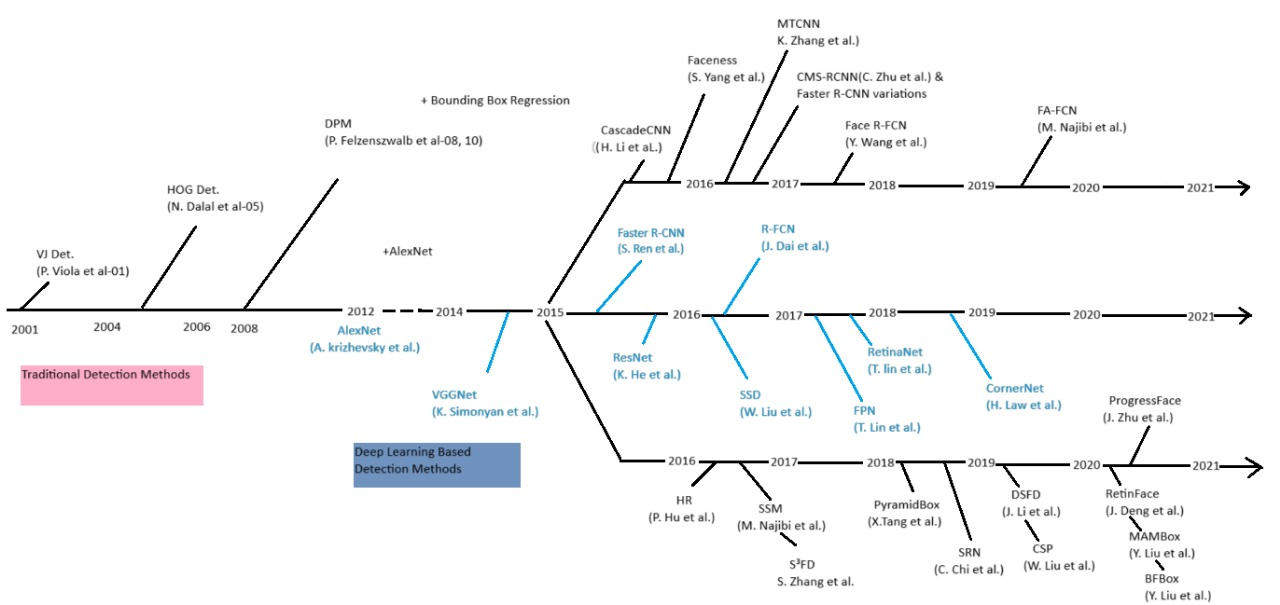
\includegraphics[width=\columnwidth]{components/images/od-timeline.jpg}}
\caption{Object Detection and Face Detection Timeline Overview}
\label{od-timeline}
\end{figure}

Several methods and frameworks, like Viola-Jones \cite{sumanto_viola-jones_2022}, \cite{rani_face_2022}, HOG \cite{rani_face_2022}, MTCNN \cite{rani_face_2022}, MobileNet-SSD \cite{chan_face_2022}, and YOLO-Face \cite{wang_yolov5s-face_2022}, have been utilized to ensure consistent face detection in varying conditions. Once the face is extracted, recognition involves comparing faces within a certain range or threshold, with techniques like PCA and ICA used for accuracy. Lightweight model advancements, such as those based on lightweight models like GhostNet \cite{alansari_ghostfacenets_2023}, have also been explored to meet computational demands for lower end devices.

Authors in \cite{sumanto_viola-jones_2022} used ViolaJones method's on WIDER FACES dataset and achieved a 100\% success rate on detection in groups and meetings, while the previous approaches only managed the highest accuracy results were obtained at 90.9\% for facial images and 75.5\% for non-face images. While these approaches are good under controlled environments their accuracy decreases in uncontrolled environments. Exploring the challenges of detecting faces in uncontrolled environments with varying poses, addressing shortcomings caused by environmental factors, lighting conditions, and image quality authors in \cite{mahesh_smart_2022} proposed an 8-layer Alexnet Convolutional Neural Network (ACNN). By comparing ACNN with the Support Vector Machine (SVM), the research demonstrates that ACNN outperforms SVM, achieving a remarkable 96\% accuracy compared to SVM's 89\% in recognizing faces with varying poses.

Multitask-Net model proposed in \cite{viet_simultaneous_2021} overcomes the challenges of face detection and head pose estimation in digital images which is vital for applications like surveillance. The authors enhances head pose estimation accuracy by leveraging features from face detection and predicts head position and direction simultaneously, utilizing Rotation matrix vectors for face orientation representation to overcome limitations. The results showcase the model's high accuracy, comparable to state-of-the-art methods.

Addressing the issues of missed and false face detection Yongwang Wand et al. \cite{wang_yolov5s-face_2022} proposed a new model based on YOLOV5s by modifying the anchor box size using K-means clustering, embedding an SE attention module on the backbone of YOLOV5s and adding four-scale feature detection for small target faces. This new model gained 3.9\% in mAP and 4.0\% in Recall compared to YOLOV5s. In another paper by Aifian Adi Sufian et al. \cite{chan_face_2022} introduces a two-step face detection framework designed to reduce over-detection in face images and misdetection in non-face images. The method combines feature detection using SSD MobileNet V2 and a geometrical algorithm. When compared to leading algorithms the approach achieved a 91.5\% prediction accuracy. Although it didn't surpass MTCNN and Dlib in accuracy, it was superior in minimizing both over-detection and misdetection.

Farooq et al. \cite{farooq_hybrid_2021} highlights the challenges posed by variations in age, lighting, expressions, and image quality, especially for individuals with dark skin, where existing algorithms tend to perform poorly. To address this racial disparity in facial recognition technology, the authors presents a hybrid algorithm combining Gaussian Model and Explicit Rule Algorithm for skin detection. This innovative approach significantly improves the face detection accuracy for dark-skinned individuals by an impressive 89\%. This underscores the importance of diverse training datasets.

Night time video surveillance arising from varying environmental light conditions can lead to underexposed distant objects and overexposed nearby objects. To combat these issues, the authors in \cite{lu_fusion_2022} introduces the concept of a multi-intensity IR illuminator with periodically varying intensity. The MI3 database is established to assess object detectors in different scenes and illuminations. It evaluates human and face detectors, presenting satisfactory results for simple scenes and proposing a baseline approach for fusion among different illumination intensities.

Khalid M et al. \cite{hosny_privacy_2022} addresses the pressing need for privacy protection in surveillance videos, given the ubiquity of surveillance cameras in our lives. It focuses on safeguarding sensitive regions, particularly people's faces, within surveillance footage. The proposed method employs an object detector, YOLOv3 \cite{aziz_exploring_2020}, to identify the regions and subsequently applies a fast block scrambling technique for obfuscation. Encryption is then applied using secret keys generated from a chaotic logistic map. Notably, the method extends protection to the edges of detected regions to prevent sensitive information leakage. This approach offers practical and robust privacy protection for surveillance videos, ensuring the confidentiality of sensitive data and resilience against potential attacks.

While convolutional neural networks (CNNs) or other Deep learning based approaches have shown promise in face detection, their computational demands can be prohibitive, especially for CPU-based systems as it also adds to the computational complexity and thus requires good hardware which is often not the case with real time surveillance systems, the critical need for lightweight and efficient face detection methods without compromising accuracy was addressed by Muhamad Dwisnanto Putro et al \cite{putro_high_2021}. The authors introduces an optimized architecture, featuring a lightweight CNN with two key modules: a feature extraction backbone and a multilevel detector for accommodating scale variations in face detection. With less than a million parameters, this novel method produces state-of-the-art performance among CPU-based real-time detectors, operating at an astounding 53 frames per second (FPS).

\section{Face Tracking} \label{section:ft}
A face tracker is a computer vision system or algorithm designed to locate and follow a face in a sequence of frames or a video stream. The primary goal of face tracking is to maintain the identity of a face over time, regardless of facial movements, rotations, occlusions, or changes in facial expressions. Several technologies and algorithms, ranging from classical computer vision techniques to deep learning models, can be used in face tracking. A comprehensive survey of Siamese trackers in visual object tracking (a parent field of face tracking) was done by Milan Ondrasovic et al \cite{ondrasovic_siamese_2021}. Siamese trackers leverage deep learning and similarity learning for tracking objects in videos. They tackle challenges like scale and lighting variations, occlusion, and background clutter. According to authors recent trends involve using deeper backbones like ResNet \cite{aziz_exploring_2020}, multi-level feature fusion, and template updating strategies for improved performance. Cross-correlation with attention mechanisms has shown promise in achieving a balance between speed and accuracy.

Kim et al. \cite{kim_facial_2023} while developing a real time face recognition system used deepSORT as the tracking module. SORT (Simple Online and Realtime Tracking) is to provide a computationally efficient and straightforward method for tracking objects, especially in real-time scenarios. While SORT is computationally efficient and suitable for real-time scenarios, it's primarily designed for scenarios where the number of objects remains relatively constant, and there are minimal interactions or occlusions among objects. For more complex scenarios with numerous occlusions, interactions, and variable object counts, more sophisticated algorithms like DeepSORT (which augments SORT with deep learning-based features).

In real-time face recognition systems, multi-face tracking in unconstrained films is crucial for identifying and preserving the identities of numerous faces throughout time. \cite{weng_online_2023} presented a two-stage framework for an online multi-face tracking approach that includes detection alignment and detection association. To create tracking trajectories, it aligns face and body detections and compares the matched detections with characteristics found on the face or body. Trials on reference datasets show that tracking performance is much improved by combining both body and face information as opposed to only face data, which puts it on par with or better than previous online tracking techniques for multi-face tracking. An alternative method for video surveillance presents a cross-camera multi-face tracking system \cite{ren_cross-camera_2021}. It combines the Chinese Whisper face clustering algorithm and Double Triplet Networks (DTN) to accurately track pedestrians' faces across different cameras. Experimental results demonstrate its effectiveness, achieving a recognition accuracy of 99.51\% with the DTN MSML Batch OHNM Subspace FOCAL LOSS model. It addresses challenges like small target tracking and occlusion, offering a robust solution for efficient face tracking in surveillance scenarios.

Face tracking in crowded scenes presents a myriad of challenges, central to which is the issue of occlusions where faces are frequently obscured by other individuals or objects. Such environments often result in overlapping faces, making distinct identification and continuous tracking a daunting task. Authors in \cite{barquero_rank-based_2021} focused on enhancing video surveillance systems in crowded and unconstrained scenarios and introduces a novel tracklet reconnection strategy, utilizing rank-based face verification, to extend track lengths by up to 50\% compared to deep learning trackers. This constraint method also reduces identity mixing errors and improves completion rates.

Vivek Sharma et al. \cite{sharma_video_2020} tackled the problems of video face clustering in the context of growing variety in facial appearance. They presented self-supervised Siamese networks and deep pre-trained face networks as unsupervised techniques for feature refining. As a robust generative model baseline, discriminative models such as Track-supervised Siamese Network (TSiam) and Self-supervised Siamese Network (SSiam) are suggested in conjunction with Variational Autoencoders (VAEs). The algorithms outperform current state-of-the-art techniques when tested on difficult video face clustering datasets. The models' computational efficiency, according to the authors, makes them appropriate for a variety of appearance datasets.

\section{Face Recognition} \label{section:fr}
Facial recognition systems generally follow a three-step approach: face detection \ref{section:fd}, face tracking \ref{section:ft}, feature extraction, and identification or verification. While deep learning techniques have significantly improved facial recognition performance, achieving accuracy rates over 99\% on certain datasets, there are concerns about their real-world applicability, especially when recognizing individuals intent on avoiding detection \cite{kim_surveillance_2023}.

Face recognition starts with extracting the face area and its features, which can be a classification challenge to determine if the detected section is a face.

Facial recognition in videos can present ethical dilemmas, particularly in mistakenly identifying innocent bystanders. Most surveillance cameras record at 15 FPS due to storage constraints, but can capture at faster rates. Videos, which provide higher-dimensional data than static images, often give fragmented insights.

Authors in \cite{zhu_webface260m_2023} presents WebFace260M benchmark dataset, WebFace42M benchmark dataset and the Face Recognition Under Inference Time conStraint (FRUITS) protocol for comprehensive evaluation and addresses biased face recognition deployments, including masked and unbiased scenarios. 

Kim et al. \cite{kim_facial_2023} proposed a real-time Criminal Recognition system with 2 major update one is down sampling the input image for reducing the latency during the face detection, whereas high identification accuracy is maintained during the identification step by cropping the face regions from the original high-resolution images. The addition of Score Dictionary Identification was another improvement. This method involves building a dictionary using the tracking ID as a key and adding scores relevant to the identification results for each monitored face's face ID. The dictionary keeps track of the score so that when it rises beyond a certain level, the system sends out an identification result and the criminal's picture.

\subsection{For Devices with limited Computational Power}

Alansari et al. \cite{alansari_ghostfacenets_2023} proposed a deep learning biometric models suitable for devices with limited memory and computational power by the introduction of Ghost modules marks a significant advancement. The model was named GhostFaceNets, lightweight face recognition models, are built upon GhostNetV1 and GhostNetV2, both rooted in Ghost modules. GhostFaceNets, when trained using the ArcFace loss on the refined MS-Celeb-1M dataset, showcased leading performance across benchmarks. They significantly boost efficiency in face verification compared to earlier top mobile CNNs. GhostFaceNets greatly improve efficiency for face verification tasks compared to previous SOTA mobile CNNs, making them suitable for deployment on devices with constrained memory and computational resources. In another such paper \cite{abuzneid_enhanced_2018} authors used back-propagation neural network (BPNN) and correlation-based feature extraction to improve face recognition accuracy. The proposed method achieves higher accuracy with reduced computational cost by generating a new set called the T-Dataset and using a local binary pattern histogram descriptor.

\subsection{Homogeneous Face Recognition}

Homogeneous Face Recognition generally refers to scenarios where the recognition system is designed to handle specific variations or challenges, such as age, pose, lighting, or expression.

With the advent of Covid-19 pandemic a new challenge for face recognition arise which was Masked Face Recognition. Given the global health circumstances since 2020 and the widespread adoption of face masks, masked face recognition has become a notable subfield within Homogeneous Face Recognition, addressing the unique challenges introduced by facial coverings.The authors \cite{9914874} suggested a masked facial recognition algorithm that combines Support Vector Machine (SVM) and Convolutional Neural Network (CNN): SVM is used as a label classification technique, while CNN is utilised to train the model. The studies employ two benchmarked datasets: the Labelled Face in The Wild Simulated Masked Face Dataset (LFW-SMFD) and the Real World Masked Face Dataset (RMFD). The suggested approach shows promise in identifying unconstrained face photos with a 98.39 percent true acceptance rate on RMFD and 94.29 percent on LFW-SMFD. Pedro Neto et al. \cite{pedro_neto_beyond_2022} accessed the performance of MFR algorithms was assessed on both masked and occluded face datasets. This assessment was again repeated using a top-performing occluded face recognition algorithm. Finally, to understand the broader context, the evaluation was again performed using algorithms intended for general face recognition. The authors evaluate several approaches for handling masks, including unmasking the input image, unmasking the template generated by a face recognition model, and using a model that is robust to masks.

Age significantly impacts face recognition due to the natural morphological changes that occur over time. Age-related factors can introduce intra-class variations that may pose challenges to recognition algorithms. Age-Invariant Model (AIM) \cite{zhao_towards_2022} was proposed for face recognition in the wild. The model performs cross-age face synthesis and recognition jointly. The AIM model achieves continuous face rejuvenation/aging with photorealistic and identity-preserving properties, without the need for paired data or the true age of testing samples.

\subsection{Heterogeneous Face Recognition}

One other field of face recognition is Heterogeneous Face Recognition (HFR) which refers to the task of matching faces across different domains or modalities. It involves matching a near-infrared (NIR) facial image with a visible light facial image, a sketch of a face with a photographic image, or a thermal image of a face with a regular visible spectrum image etc. To address the heterogeneous facial recognition (HFR) challenge, a Dual variational generation (DVG-facial) \cite{fu_dvg-face_2022} framework is used. It uses a dual variational generator to learn the joint distribution of paired heterogeneous pictures and formulates HFR as a dual generation issue. To guarantee the identity consistency of the resulting paired heterogeneous pictures, a pairwise identity preservation loss is applied to them. The HFR network is trained using the produced paired heterogeneous pictures using a contrastive learning method, producing both discriminative and domain-invariant embedding features. On seven difficult datasets from five HFR tasks (NIR-VIS, Sketch-Photo, Profile-Frontal Photo, Thermal-VIS, and ID-Camera), DVG-Face beats the state-of-the-art techniques.
Graph Convolutional Autoencoder (GCA) for encoding 3D faces into latent representations, Generative Adversarial Network (GAN) for converting expressive faces' latent representations into neutral faces' latent representations, and identity recognition sub-network for 3D face recognition using the neutralised latent representations are the three components of the approach proposed by Decheng Liu et al. \cite{liu_heterogeneous_2022}. In the areas of 3D facial recognition and expression neutralisation, this has real-world applications. It provides a way to anticipate the identities of characters and produce realistic 3D faces with neutral emotions.
For Heterogeneous Face Synthesis, Identity-Attribute Disentanglement (FSIAD) \cite{yang_heterogeneous_2022} Identity-attribute disentanglement (IAD) and the face synthesis module (FSM) are the two primary phases in face recognition. In order to reduce the correlation between identities and attributes, face images are divided into identity-related representations and identity-unrelated representations (attributes) in the IAD step. The FSM is then used to generate a large number of images with stochastic combinations of identities and attributes that have been disentangled, enhancing the attribute diversity of synthetic images.

\section{Datasets} \label{section:datasets}

Datasets play a crucial role in the development, training, and evaluation of face detection and recognition systems. They provide researchers with rich resources such as transfer learning where large face datasets can be used to pre-train models, which can then be fine-tuned on smaller, task-specific datasets is often results in better performance than training on the smaller dataset alone.

Requirements of a good dataset are as follows:

\begin{enumerate}
    \item \textbf{Diversity}: The dataset should encompass a wide variety of facial features, expressions, angles, and occlusions. This ensures that the trained models generalize well to real-world scenarios.

    \item \textbf{High Quality Images}: Images should be of high resolution and clarity. Blurry or low-quality images can hinder the performance of detection or recognition systems.

    \item \textbf{Varied Lighting Conditions}: It should include faces under different lighting conditions - from well-lit to poorly lit scenarios - to challenge and enhance the robustness of algorithms.

    \item \textbf{Age Variability}: Faces from different age groups, ranging from infants to the elderly, should be represented to ensure age-invariance in recognition.

    \item \textbf{Demographic Diversity}: A balanced representation of various ethnicities, genders, and backgrounds is essential to prevent biases in the resulting models.

    \item \textbf{Annotations}: Precise annotations, including bounding boxes for detection and identity labels for recognition, are crucial.

    \item \textbf{Temporal Data}: For video-based recognition systems, the dataset should include video sequences to account for temporal variations and movements.

    \item \textbf{Real-world Scenarios}: Inclusion of "in-the-wild" images or videos where faces are naturally occluded, or in varied expressions and postures, simulates real-world challenges.

    \item \textbf{Scalability}: A good dataset should be large enough to train deep learning models, which often require vast amounts of data.

    \item \textbf{Consent and Ethics}: All data should be collected with proper consent, ensuring the privacy and rights of the individuals are respected.
\end{enumerate}



WebFace260M benchmark \cite{zhu_webface260m_2023}, an ultra-large-scale dataset comprising 4 million identities and 260 million faces was introduced to bridge the data gap between academia and industry. The dataset was still refined by employing the Cleaning Automatically by Self-Training (CAST) pipeline,into WebFace42M, with 2 million identities and 42 million faces. The benchmark and cleaned dataset facilitate efficient model training, resulting in improved face recognition performance and potential solutions for bias mitigation and privacy concerns in the field. The benchmark and cleaned dataset facilitate efficient model training, resulting in improved face recognition performance and potential solutions for bias mitigation and privacy concerns in the field.

Three different kinds of masked face datasets are proposed by Zhongyuan Wang et al. \cite{wang_masked_2023}: the Masked Face Detection Dataset (MFDD), the Real-world Masked Face Recognition Dataset (RMFRD), and the Simulated Masked Face Recognition Dataset (SMFRD). The authors assert that the Real-world Masked Face Recognition Dataset (RMFRD) is the biggest real-world masked face dataset available. Despite this, the sources given do not go into depth on the precise techniques utilised to create the datasets. The DVG-Face framework \cite{fu_dvg-face_2022} was assessed using seven difficult datasets from five HFR tasks: NIR-VIS, Sketch-Photo, Profile-Frontal Photo, Thermal-VIS, and ID-Camera. It outperforms state-of-the-art techniques and produces better results. In order to support research on age-invariant face recognition for their AIM model, Zhao et al. \cite{zhao_towards_2022} assembled a new, extensive Cross-Age Face Recognition (CAFR) benchmark dataset. In-depth tests are carried out on the CAFR dataset as well as additional cross-age datasets (MORPH, CACD, FG-NET) to show how much better the suggested AIM model is than current methods. To confirm that the AIM model can generalise to face recognition in the wild, it is further tested on unconstrained face recognition datasets (YTF, IJB-C).

Authors in \cite{abuzneid_enhanced_2018} used 3 datasets YALE and AT\&T for testing the proposed framework and evaluated their method on the LFW dataset, which is a state-of-the-art benchmark dataset for face recognition.

When the model is used in an uncontrolled environment with noise, occlusion, external lighting, cosmetics, etc.—sometimes referred to as "in the wild"—accuracy decreases. Detection in a controlled setting frequently yields excellent results. However, these sorts of photos are present in datasets. A dataset of this kind is the WIDER FACE dataset, which is used in \cite{putro_high_2021} as a training dataset for the CNN-based lightweight detector. Of the 32,203 photos in it, 12,800 were utilised especially to train the detector. In order to minimise overfitting and enhance the training data, augmentation methods are used. The second dataset has 851 photos with 1335 tagged faces and is called the PASCAL face dataset \cite{putro_high_2021}. This dataset, which is an indoor and outdoor subset of the PASCAL VOC dataset, including changes in backdrop and stance.

Datasets like VGGFace2 and MS-Celeb-1M, which primarily contain data from young, facially beautiful celebrities with makeup, are biased in terms of age and facial appearance, leading to potential performance issues when using pretrained models from these datasets on different audiences \cite{wanyonyi_open-source_2022}.

Tables \ref{det-ds} and \ref{rec-ds} contains a list of popular publicly available datasets found in the literature survey:

\begin{table}[htbp]
\caption{Detection Datasets}
\begin{center}
\begin{tabularx}{\columnwidth}{|X|c|X|}
\hline
\textbf{Dataset} & \textbf{Year}& \textbf{Size} \\
\hline
VGGFace2 \cite{kim_face_2022} & 2018 & 3.31 million images of 9,131 subjects \\
\hline
WIDER Face \cite{kim_face_2022} & 2016 & 32,203 images with 393,703 annotated face bounding boxes \\
\hline
VGGFace2 \cite{kim_face_2022} & 2018 & 3.31 million images of 9,131 subjects \\
\hline
PASCAL Face \cite{feng_detect_2022} & 2012 & 1,335 faces from 851 images \\
\hline
\end{tabularx}
\label{det-ds}
\end{center}
\end{table}
    
    
\begin{table}[htbp]
\caption{Recognition Datasets}
\begin{center}
\begin{tabularx}{\columnwidth}{|X|c|X|}
\hline
\textbf{Dataset} & \textbf{Year}& \textbf{Size} \\
\hline
MS-Celeb-1M \cite{wanyonyi_open-source_2022} & 2016 & 10 million images of 100,000 celebrities \\
\hline
LFW \cite{kim_face_2022} & 2007 & 13,000 images of 5,749 distinct individuals \\
\hline
CASIA NIR-VIS 2.0 \cite{liu_heterogeneous_2022} & 2007 & 17,580 images from 725 subjects \\
\hline
ChokePoint \cite{barquero_rank-based_2021} & 2011 & 54 video sequences captured from 6 different camera views \\
\hline
\end{tabularx}
\label{rec-ds}
\end{center}
\end{table}

\section{Proposed System}
The core of the proposed system is a real-time face recognition engine that encompasses multiple components: face detection, face tracking, face encoding, and identification. The system will leverage state-of-the-art algorithms, deep learning methodologies, and vast datasets to ensure optimal accuracy and speed, even in challenging scenarios encountered by law enforcement agencies. This engine integrates seamlessly with a database of known individuals and offers a user-friendly interface for law enforcement personnel. At its core, the system is engineered to overcome the challenges inherent in the real time face recognition scenarios, including occlusion handling, dynamic background, crowded scenarios etc. This proposed system consists of a set of cutting-edge components and features that collectively redefine the real time face recognition:

	\subsection{Face Detection Module}
		The face detection module prioritizes real-time processing and emphasizes rotation invariance and region-of-interest determination. The primary task is to have capability to process live video feeds instantly. As it's a real time video stream so the latency should be pretty low and the detection accuracy should be high. This is the heart of the entire architecture as without detection there is no point of recognition so the detection module should be fast and accurate to identify the faces in the wild where there are challenges like occlusion, dynamic background and heavy crowd etc. The module in order to ace encompasses deep learning-based algorithms like RetinaFace, YOLO or SSD for rapid and accurate detection of faces in images or video streams as they are the current state of the art algorithms. It prioritizes regions in a frame with higher chances of containing faces, optimizing computational resources. It also incorporates multi-scale detection to capture faces of varying sizes and at different distances from the camera.
		The face detection module employs advanced algorithms to detect faces in the wild.
		

	\subsection{Face Tracking Module}
		As faces are detected, they are tracked over time using a sophisticated module that ensures temporal consistency, can simultaneously track multiple faces in crowded scenarios, and employs predictive pathing to anticipate movements. For this advanced tracking algorithms such as deepSORT or Siamese networks are employed. They are designed to maintain continuous tracking, even when the subject moves, turns their face, or gets partially obscured. The main task is to predicts and anticipates the path a face might take, ensuring smoother tracking.

	\subsection{Face Encoding and Identification Module}
		Once tracked, faces undergo deep feature extraction within the identification module that matches them rapidly against a vast database while employing anti-spoofing techniques. This module extracts facial features and converts them into a compact vector (or embedding) using neural networks like ResNet or VGG. Then it compares the derived embeddings with a database of known embeddings to ascertain identity. As there would always be some faces that will be probable the module integrates a threshold mechanism to eliminate false positives and ensure high-confidence identifications. Once the module is confident enough an alert will be generated and given to the respective authorities about the detection.

	\subsection{Database Integration}
		The system seamlessly integrates with an encrypted, secure, and fast-access database storing facial embeddings of known individuals. This way they incorporates a periodic update mechanism to add new embeddings and ensure the database remains current. It would incorporate a tagging mechanism to efficiently tag and categorize faces for quicker searches. Regular backups should also be taken to prevent data loss and facilitate recovery. The system's database structure prioritizes differential updates, ensuring minimal lag.

	\subsection{Training and Update Mechanism}
		The proposed system suggests instead of complete retraining, the training should be incremental and the thus updates the model with new data increments only. The model evaluation should also be automated and continuous evaluation of model performance and automatic rollback should be done if a newer version performs poorly. It also Incorporate feedback from users to refine and improve models.

	\subsection{Performance Analytics}
		The reports should be customizable to suit specific requirements and real-time alerts should be given for any anomalies or performance drops. The module provides trends and historical data for long-term performance assessment.
		
	\subsection{Cross-Platform Accessibility}
		The proposed system is designed with accessibility in mind. It is accessible across various platforms, including web browsers, mobile applications, and other embedded devices. This cross-platform approach ensures that users can engage with the system on their preferred devices, making it versatile and user-friendly.